\documentclass{article}

\usepackage[a4paper, margin=2cm]{geometry}
\usepackage{tikz-qtree}
\usepackage{enumitem}
\usepackage{bussproofs}
\usepackage{titlesec}

\titleformat*{\section}{\Large\bfseries}
\titleformat*{\subsection}{\large\bfseries}
\titleformat*{\subsubsection}{\normalsize\bfseries}
\titleformat*{\paragraph}{\normalsize\bfseries}
\titleformat*{\subparagraph}{\normalsize\bfseries}
\setlength\parindent{0pt}

\begin{document}

\Large\textbf{PROBLEM SET 2: SYNTAX} \\
\normalsize
Alice McKean \\
\today

\section{Tree Drawing}
\large\textbf{1.1: Deep Structure} \\
\hfill \break
\begin{tikzpicture}[scale=0.9, transform shape]
\Tree [.CP [.C Q+ ]
           [.IP [.NP [.N Harkim ] ]
                [.I  [.[Past] ] ]
                [.VP [.V know ]
                     [.CP [.C if ]
                          [.IP [.NP [.N they ] ]
                               [.I  [.[Past] ] ]
                               [.VP [.VP [.V invite ]
                                         [.NP [.N Lea ] ]
                                    ]
                                    [.PP [.P to ]
                                         [.NP [.D the ]
                                              [.N party ]
                                         ]
                                    ]
                               ]
                          ]
                     ]
                ]
           ]
      ]
\end{tikzpicture} \\
\hfill \break
\large\textbf{1.1: Surface Structure} \\
\hfill \break
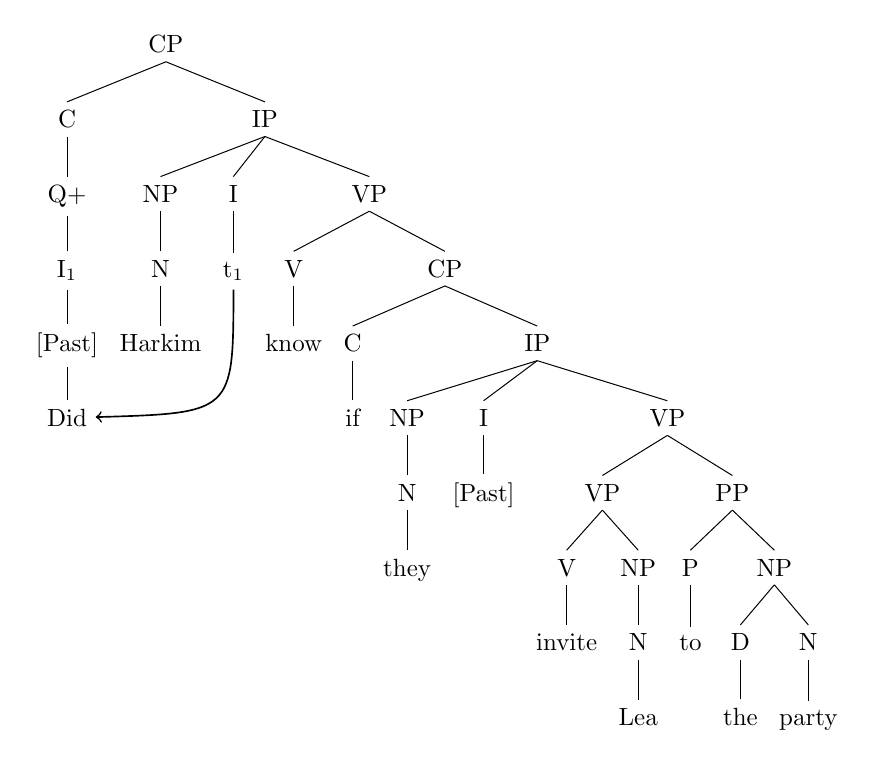
\begin{tikzpicture}[scale=0.9, transform shape]
\Tree [.CP [.C  [.Q+ [.I$_1$ [.[Past] \node(do){Did}; ] ] ] ]
           [.IP [.NP [.N Harkim ] ]
                [.I \node(t){t$_1$}; ]
                [.VP [.V know ]
                     [.CP [.C if ]
                          [.IP [.NP [.N they ] ]
                               [.I  [.[Past] ] ]
                               [.VP [.VP [.V invite ]
                                         [.NP [.N Lea ] ]
                                    ]
                                    [.PP [.P to ]
                                         [.NP [.D the ]
                                              [.N party ]
                                         ]
                                    ]
                               ]
                          ]
                     ]
                ]
           ]
      ]
\draw[semithick,->] (t)..controls +(south:2)..(do);
\end{tikzpicture}

\newpage

\large\textbf{1.2: Deep Structure} \\
\hfill \break
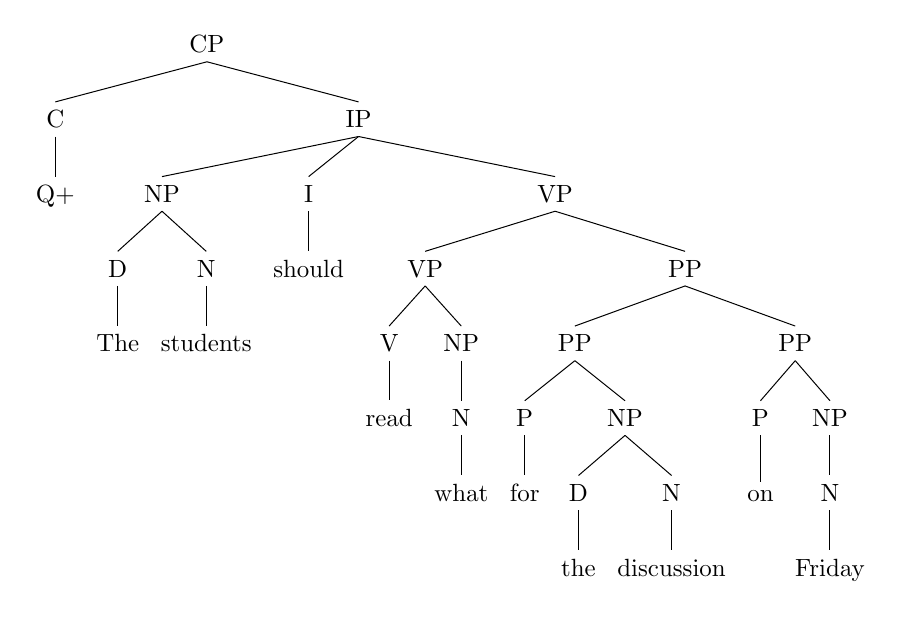
\begin{tikzpicture}[scale=0.9, transform shape]
\Tree [.CP [.C Q+ ]
           [.IP [.NP [.D The ]
                     [.N students ]
                ]
                [.I  should ]
                [.VP [.VP [.V read ]
                          [.NP [.N what ] ]
                     ]
                     [.PP [.PP [.P for ]
                               [.NP [.D the ]
                                    [.N discussion ]
                               ]
                          ]
                          [.PP [.P on ]
                               [.NP [.N Friday ] ]
                          ]
                     ]
                ]
           ]
      ]
\end{tikzpicture} \\
\hfill \break
\large\textbf{1.2: Surface Structure} \\
\hfill \break
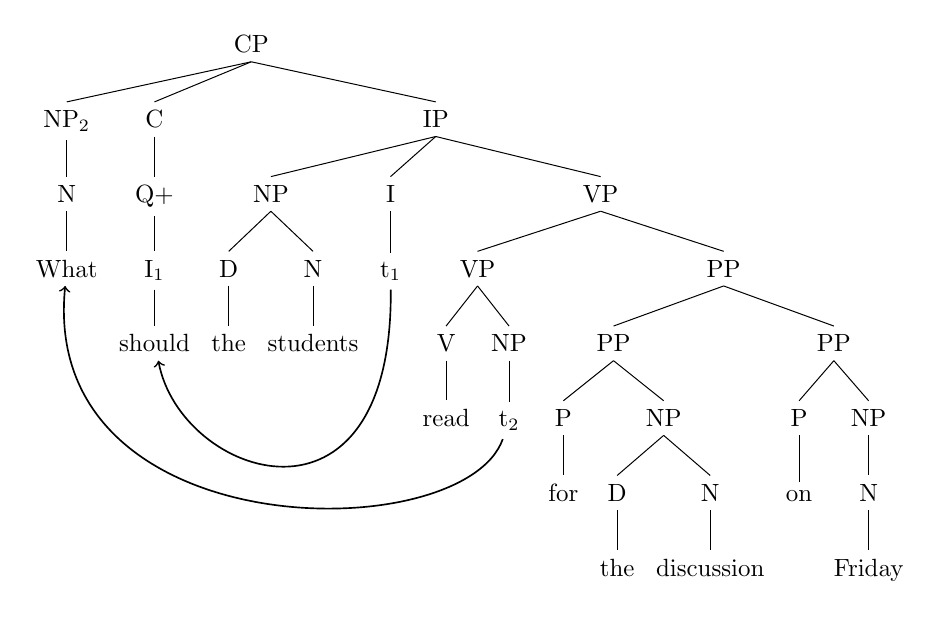
\begin{tikzpicture}[scale=0.9, transform shape]
\Tree [.CP [.NP$_2$ [.N \node(wh){What}; ] ]
           [.C  [.Q+ [.I$_1$ \node(aux){should}; ] ] ]
           [.IP [.NP [.D the ]
                     [.N students ]
                ]
                [.I  \node(t1){t$_1$}; ]
                [.VP [.VP [.V read ]
                          [.NP \node(t2){t$_2$}; ]
                     ]
                     [.PP [.PP [.P for ]
                               [.NP [.D the ]
                                    [.N discussion ]
                               ]
                          ]
                          [.PP [.P on ]
                               [.NP [.N Friday ] ]
                          ]
                     ]
                ]
           ]
      ]
\draw[semithick,->] (t1)..controls (2,-7) and (-1,-6)..(aux);
\draw[semithick,->] (t2)..controls (3,-7) and (-3,-7)..(wh);
\end{tikzpicture}

\newpage

\large\textbf{1.3: Deep Structure} \\
\hfill \break
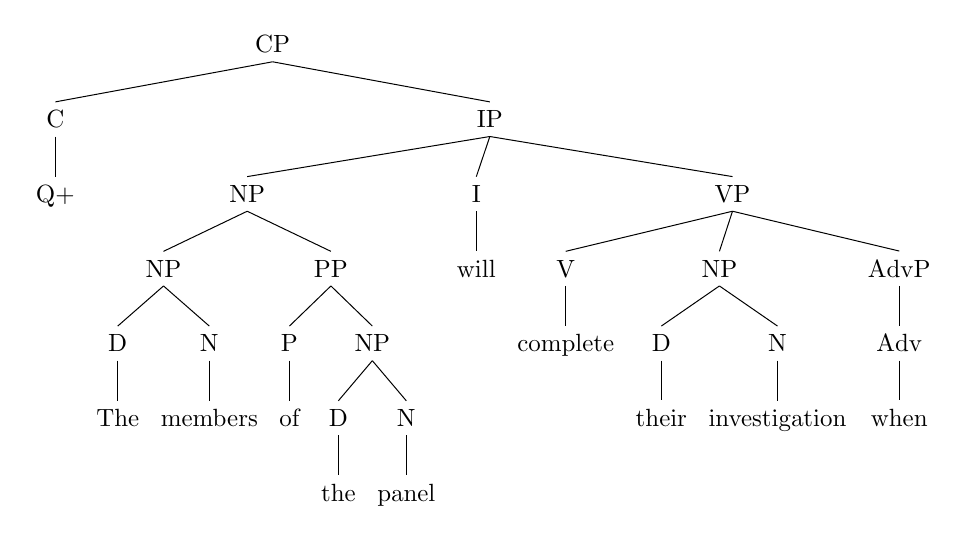
\begin{tikzpicture}[scale=0.9, transform shape]
\Tree [.CP [.C Q+ ]
           [.IP [.NP [.NP [.D The ]
                          [.N members ]
                     ]
                     [.PP [.P of ]
                          [.NP [.D the ]
                               [.N panel ]
                          ]
                     ]
                ]
                [.I  will ]
                [.VP [.V complete ]
                     [.NP [.D their ]
                          [.N investigation ]
                     ]
                     [.AdvP [.Adv when ] ]
                ]
           ]
      ]
\end{tikzpicture} \\
\hfill \break
\large\textbf{1.3: Surface Structure} \\
\hfill \break
\begin{tikzpicture}[scale=0.9, transform shape]
\Tree [.CP [.AdvP$_2$ [.Adv \node(wh){When}; ] ]
           [.C  [.Q+ [.I$_1$ \node(aux){will}; ] ] ]
           [.IP [.NP [.NP [.D the ]
                          [.N members ]
                     ]
                     [.PP [.P of ]
                          [.NP [.D the ]
                               [.N panel ]
                          ]
                     ]
                ]
                [.I  \node(t1){t$_1$}; ]
                [.VP [.V complete ]
                     [.NP [.D their ]
                          [.N investigation ]
                     ]
                     [.AdvP \node(t2){t$_2$}; ]
                ]
           ]
      ]
\draw[semithick,->] (t1)..controls (4,-11) and (-2, -11)..(aux);
\draw[semithick,->] (t2)..controls (8,-12) and (-4, -14)..(wh);
\end{tikzpicture}

\newpage

\large\textbf{1.4: Deep Structure} \\
\hfill \break
\begin{tikzpicture}[scale=0.9, transform shape]
\Tree [.CP [.C Q- ]
           [.IP [.NP [.N They ] ]
                [.I  might ]
                [.VP [.V know ]
                     [.CP [.C Q+ ]
                          [.IP [.NP [.N Darya ] ]
                               [.I  [.[Pres] ] ]
                               [.VP [.VP [.V relies ]
                                         [.PP [.P on ]
                                              [.NP [.D which ]
                                                   [.N informants ]
                                              ]
                                         ]
                                    ]
                                    [.PP [.P for ]
                                         [.NP [.N information ] ]
                                    ]
                               ]
                          ]
                     ]
                ]
           ]
      ]

\end{tikzpicture} \\
\large\textbf{1.4: Surface Structure} \\
\hfill \break
\begin{tikzpicture}[scale=0.9, transform shape]
\Tree [.CP [.C Q- ]
           [.IP [.NP [.N They ] ]
                [.I  might ]
                [.VP [.V know ]
                     [.CP [.C [.Q+ [.NP$_1$ [.D which ]
                                            [.N \node(wh){informants}; ]
                                   ]
                              ]
                          ]
                          [.IP [.NP [.N Darya ] ]
                               [.I  [.[Pres] ] ]
                               [.VP [.VP [.V relies ]
                                         [.PP [.P on ]
                                              [.NP \node(t1){t$_1$}; ]
                                         ]
                                    ]
                                    [.PP [.P for ]
                                         [.NP [.N information ] ]
                                    ]
                               ]
                          ]
                     ]
                ]
           ]
      ]
\draw[semithick,->] (t1)..controls (9,-12) and (5,-12)..(wh);
\end{tikzpicture}

\newpage
\section{Inference Relations}
\begin{enumerate}[label=(\theenumi)]
\setcounter{enumi}{4}
\item In this block (b) entails (a) and (b) presupposes (a) because in order for the
  kangaroo who stole the boomerang to be caught that kangaroo must have stolen
  the boomerang.
\item In this block (a) entails (b) and (a) presupposes (b) because Otto happens to be a
  someone.
\item In this block (a) entails (b) and (b) entails (a) as the three different words
  in (a) don't change the truth value of (b).
\item These sentences don't match any of the options because you can murder
  someone without poisoning them and you can poisoning someone without murdering them.
\end{enumerate}
\section{Focus and Inference Relations}
Shifting the placement of the focus does not change what the sentence entails.
The following judgments illustrate this fact.
\begin{prooftree}
\AxiomC{Kia sent the parcel on Monday.}
\UnaryInfC{The parcel was sent.}
\end{prooftree}
\begin{prooftree}
\AxiomC{Kia \textsc{sent} the parcel on Monday.}
\UnaryInfC{The parcel was sent.}
\end{prooftree}
Shifting the placement of the focus does however change what the sentence
presupposes. Wherever the speaker places the focus the speaker is presupposing
that the listerner had the wrong idea about the focus. If the listerner said
``Kia lost the parcel on Monday'' a likely response would be ``Kia \textsc{sent}
the parcel on Monday.''
\section{Movement and Presupposition}
\subsection{Factive Clauses}
\begin{enumerate}[label=\alph*.]
\item Non-Factive just because someone said something doesn't mean the thing they
  said is true.
  \begin{prooftree}
    \AxiomC{Corbin said the sky is green.}
    \RightLabel{$\times$}
    \UnaryInfC{The sky is green.}
  \end{prooftree}
\item Non-Factive because someone can think untrue thoughts.
  \begin{prooftree}
    \AxiomC{Corbin thinks the sky is green.}
    \RightLabel{$\times$}
    \UnaryInfC{The sky is green.}
  \end{prooftree}
\item Factive because under the cooperation principle in order to realize something
  it must be true. Now Corbin can see the light:
  \begin{prooftree}
    \AxiomC{Corbin realized the sky is blue.}
    \UnaryInfC{The sky is blue.}
  \end{prooftree}
\item Non-Factive for a similar reason as (b).
\item Factive because if you forgot something you must have once thought it to
  be true.
\end{enumerate}
\subsection{Factive-Wh Movement}

The following trees illustrate the structural ambiguity in the sentence
``When did Corbin say that the wombat killed the archbishop.'' The ambiguity
arises from the fact that the ``When'' trace can live at multiple levels of the
parse tree.

\newpage
\large\textbf{Parse 1} \\
\hfill\break
\begin{tikzpicture}[scale=0.9, transform shape]
\Tree [.CP [.AdvP$_2$ [.Adv \node(wh){When}; ] ]
           [.C  [.Q+ [.I$_1$ [.[Past] \node(aux){did}; ] ] ] ]
           [.IP [.NP [.N Corbin ] ]
                [.I  \node(t1){t$_1$}; ]
                [.VP [.VP [.V  say ]
                          [.CP [.Q+ ]
                               [.CP [.C that ]
                                    [.IP [.NP [.D the ]
                                              [.NP wombat ]
                                         ]
                                         [.I  [.[Past] ] ]
                                         [.VP [.VP [.V kill ]
                                                   [.NP [.D the ]
                                                        [.N archbishop ]
                                                   ]
                                              ]
                                              [.AdvP [.Adv \node(t2){t$_2$}; ] ]
                                         ]
                                    ]
                               ]
                          ]
                     ]
                ]
           ]
      ]
\draw[semithick,->] (t1)..controls (2,-7) and (-1, -7)..(aux);
\draw[semithick,->] (t2)..controls (15,-18) and (-4, -18)..(wh);
\end{tikzpicture}

\newpage
\large\textbf{Parse 2} \\
\hfill\break
\begin{tikzpicture}[scale=0.9, transform shape]
\Tree [.CP [.AdvP$_2$ [.Adv \node(wh){When}; ] ]
           [.C  [.Q+ [.I$_1$ [.[Past] \node(aux){did}; ] ] ] ]
           [.IP [.NP [.N Corbin ] ]
                [.I  \node(t1){t$_1$}; ]
                [.VP [.VP [.V  say ]
                          [.CP [.Q+ ]
                               [.CP [.C that ]
                                    [.IP [.NP [.D the ]
                                              [.NP wombat ]
                                         ]
                                         [.I  [.[Past] ] ]
                                         [.VP [.V kill ]
                                              [.NP [.D the ]
                                                   [.N archbishop ]
                                              ]
                                         ]
                                    ]
                               ]
                          ]
                     ]
                     [.AdvP [.Adv \node(t2){t$_2$}; ] ]
                ]
           ]
      ]
\draw[semithick,->] (t1)..controls (0.5,-7) and (-1.5, -7)..(aux);
\draw[semithick,->] (t2)..controls (15,-18) and (-4, -18)..(wh);
\end{tikzpicture}

\newpage
\large\textbf{Resolution}\\
\hfill\break
All the sentences with non-factive verbs follow the same structural ambiguity
pattern outlined above. The sentences with factive verbs are not structurally
ambiguous. A possible new constraint is that factive verbs generate a Q- node
outside the clause IP node. This means wh elements cant move to that node or
to a higher Q+ node. An example parse tree for the factive verb ``to realize''
is shown below. This sentence can be parsed unambigously because the Q- node
disallows parsing the ``AdvP'' inside the clause. \\
\hfill\break

\begin{tikzpicture}[scale=0.9, transform shape]
\Tree [.CP [.AdvP$_2$ [.Adv \node(wh){When}; ] ]
           [.C  [.Q+ [.I$_1$ [.[Past] \node(aux){did}; ] ] ] ]
           [.IP [.NP [.N Corbin ] ]
                [.I  \node(t1){t$_1$}; ]
                [.VP [.VP [.V  realize ]
                          [.CP [.Q- ]
                               [.CP [.C that ]
                                    [.IP [.NP [.D the ]
                                              [.NP wombat ]
                                         ]
                                         [.I  [.[Past] ] ]
                                         [.VP [.V kill ]
                                              [.NP [.D the ]
                                                   [.N archbishop ]
                                              ]
                                         ]
                                    ]
                               ]
                          ]
                     ]
                     [.AdvP [.Adv \node(t2){t$_2$}; ] ]
                ]
           ]
      ]
\draw[semithick,->] (t1)..controls (0.5,-7) and (-1.5, -7)..(aux);
\draw[semithick,->] (t2)..controls (15,-18) and (-4, -18)..(wh);
\end{tikzpicture}



\end{document}